\procTitle{Динамика и цикличность коллювиальных процессов в~Северном Приохотье}
\procAuthor{Колегов~П.\,П.}
\procEmail{kolegovpp@gmail.com}
\procOrganization{СВКНИИ ДВО РАН} \procCity{Магадан}

\makeProcTitle
\index{k@Колегов~П.\,П.}

Развитие рельефообразующих процессов на склонах гор подчиняется определенной
закономерности. В данных процессах можно выделить основные типы: обрушение,
осыпание, сползание, плоскостной смыв. Все они зависят от главного агента~---
гравитации.

Результатом этих процессов является разрушение материнских пород и перемещение
обломочного материала вниз по склону и далее водными потоками в водные бассейны
осадконакопления. Для оценки динамики переноса обломочного материала применяют
различные методы, такие как расчет скорости денудации рельефа, скорости
транспортировки обломков, определение объема сносимого материала, а также объема
стока взвешенных частиц ручьев и рек. Данные методы не позволяют полностью
провести сравнение факторов и оценить их влияние при рельефообразующих
процессах

В целях решения этой проблемы в последнее время в геоморфологии стали применять
энергетический подход для количественной оценки экзогенных процессов.

Основная концепция данного подхода была изложена К.\,С.\,Воскресенским в
монографии «Современные рельефообразующие процессы на равнинах Севера России»
[1], в которой он рассчитал объемы тепла, поступающие в грунт при образовании
криогенных морфоскульптур.

В дальнейшем методика была апробирована А.\,С.\,Кузнецовым для оценки динамики
развития горно-ледникового бассейна р.\,Актру. В своей диссертационной работе [3]
он оценил энергетикy рельефа, а именно определил количество энергии, поступающей
в результате поднятия территории, выветривания горных пород и стока
взвешенных осадков р. Актру.

В ходе полевых работ 2014\,г. в результате лихенометрического анализа нами
получены новые данные о скорости транспортировки обломочного материала в телах
коллювиальных конусов. 

Лихенометрическому методу и аспектам его применения посвящено много статей как
зарубежных, так и отечественных авторов [2, 5]. Мы перечислим только его главные
положения и полученные результаты: 1~--- диаметр таллома лишайника является
функцией времени произрастания данного организма на поверхности обломка; 2~--- пик
колонизации обломков спорами лишайников приходится на начальный момент времени
транзита обломка; 3~--- интервал жизни лишайника \emph{Rhizocarpon} sp. в регионе
исследования составляет 1,5--2,0\,тыс.\,лет, что позволяет использовать его в
качестве индекса возраста поверхности. Во время транзита обломочного чехла вниз
по склону некоторые обломки могут переворачиваться, что ведет к гибели особей,
произрастающих на них, но средний возраст всей ценопопуляции сохраняется. 

Объекты исследования располагались в северо-восточной части гор Дел-Урэкчэн
(60°25’16”\,с.\,ш., 150°58’16”\,в.\,д.) в бассейне руч.\,Дуга (см.\,ри\-су\-нок)~--- правого
притока р. Нанкала (бассейн р.\,Армань). Они представлены коллювиальными конусами
длиной от 135 до 540\,м, среднее значение~--- 295\,м; высотой от 53 до 212\,м,
среднее значение~--- 130\,м. Область питания морфо\-скульптур представлена в левом
борту площадным свалом в область стока коллювия и единичными останцами, в правом
борту – скальными выступами высотой до 20–30\,м.

\begin{figure}
  \begin{center}
    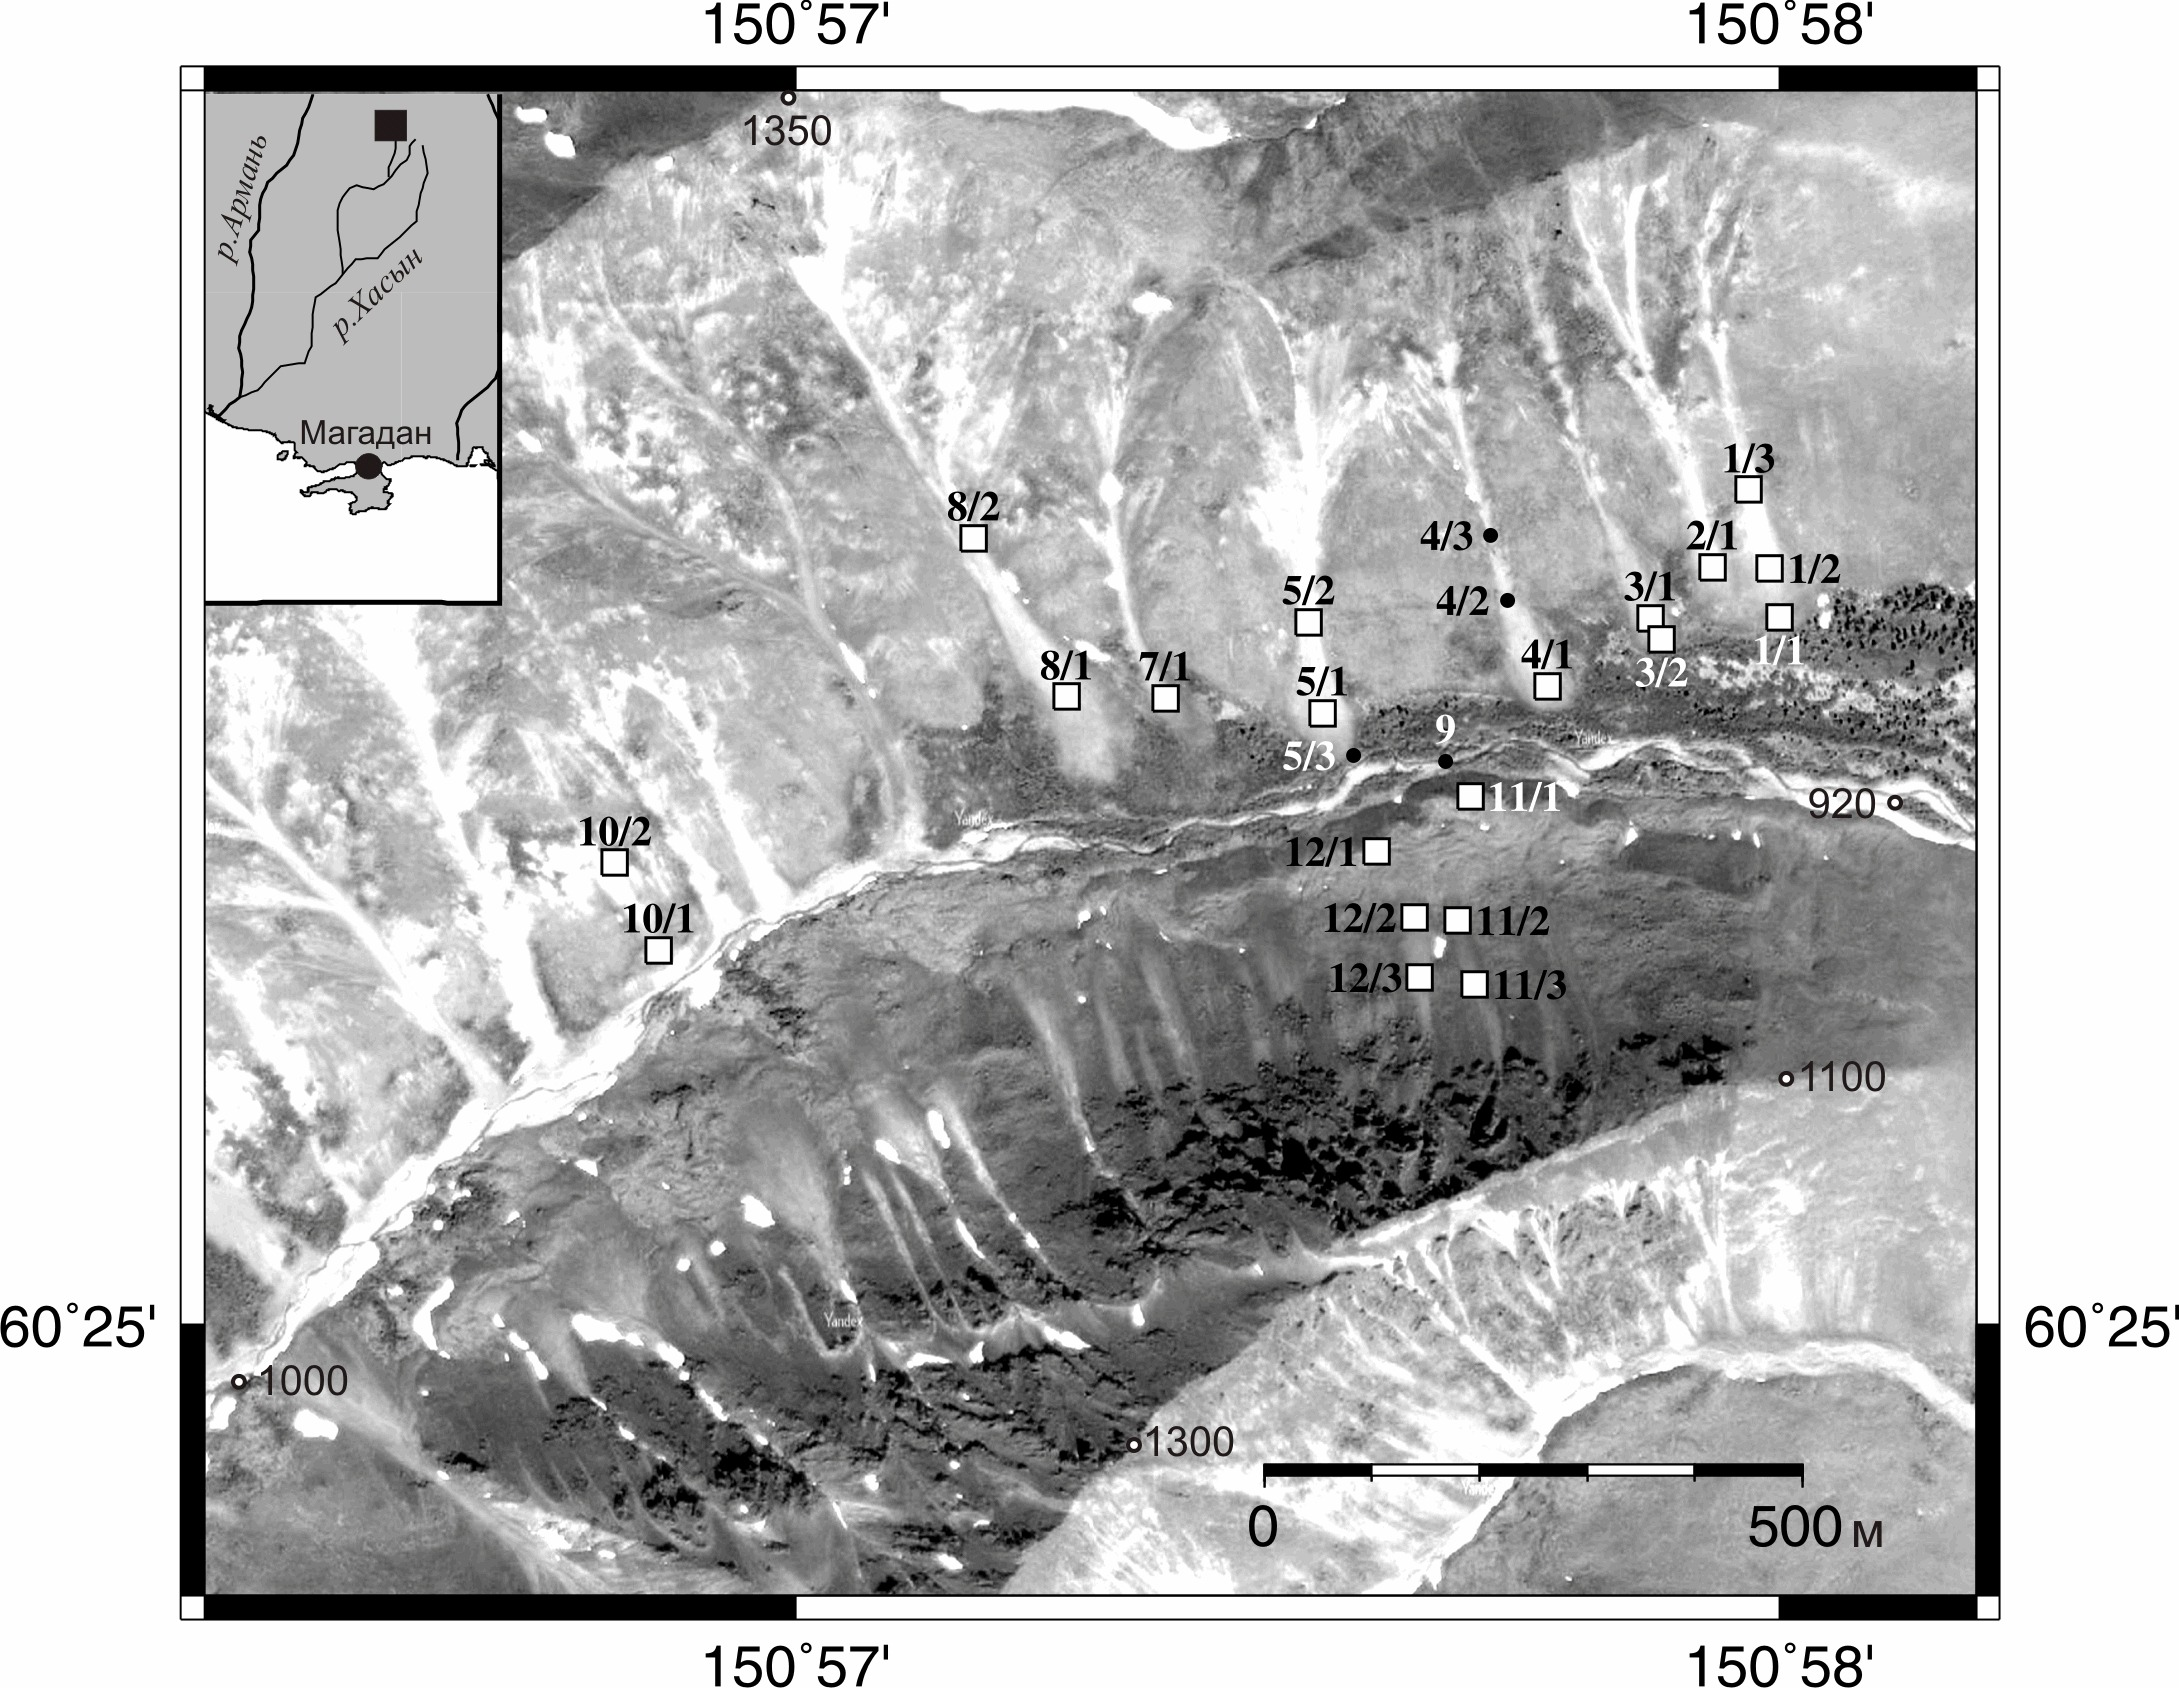
\includegraphics[width=0.9\textwidth]{authors/kolegov-fig.jpg}
  \end{center}
  \caption{Аэрофотоснимок руч.\,Дуга (горы Дел-Урэкчэн, Сев.\,Приохотье).
  Положение геолого-структурных точек наблюдений (черные точки),
  лихенометрические площадки (белые квадраты). На врезке~--- географическое
  положение района работ}
  \label{fig:kolegov}
\end{figure}


Коллювиальные конусы обладают следующими углами наклона поверхностей: транзитные
части 21–23°, аккумулятивные~--- 17–19°. Гранулометрический состав зон разгрузки
представлен, \%: щебнем средним~--- от 10 до 20, крупным~--- от 30 до 60; глыбами
мелкими~--- от 20 до 40, средними~--- от 10 до 30, крупными~--- от 2 до 10. Среднее
значение по всем изученным объектам, \%: щебня среднего~--- 10, крупного~--- 40;
глыб мелкиx~--- 30, средниx~--- 15, крупныx~--- 5.
\enlargethispage{\baselineskip}

Методика полевых работ заключалась в следующем: вдоль створа коллювиального
конуса намечался профиль. Лихенометрические площадки на профиле закладывались с
учетом петрографических и геоморфологических особенностей склона в основании, в
транзитной и верхней части. Размер площадок составлял 20\,×\,20\,м. В этих границах
проводилось измерение максимального диаметра таллома лишайника \emph{Rhizocarpon} sp.
на каждом обломке, измерению подвергались 100 обломков горных пород. Всего было
измерено примерно 2000 талломов на 20 площадках.

Для установления возраста использовали уравнение [2]:
\begin{equation}
d = a_0 f (1 - e^{\frac{-t}{f}}),
\end{equation}
где $d$~--- максимальный диаметр лишайника; $a_0$~--- коэффициент скорости роста
лишайника, равный 0,23\,мм/год, на высоте 400--800\,м\,н.\,у.\,м.; $f$~--- коэффициент
\fontdimen2\font=0.5ex
замедления роста таллома, равный 1000\,лет; $t$~--- возраст таллома.
\fontdimen2\font=\origiwspc

Скорость транспортировки обломков рассчитывали как отношение расстояния между
площадками к разности времени экспозиции данных площадок.

Для оценки динамики развития коллювиальных процессов, в частности осыпных, мы
использовали новый подход, а именно метод энергетической эффективности
рельефообразующих процессов [4]. Данный метод позволяет рассчитать затраченную
энергию на формирование объектов исследования и выразить ее в джоулях, а также
выполнить сравнительный анализ с другими типами рельефообразующих процессов.

Расчет энергетической эффективности (энергетического потенциала) проводили по
следующей формуле [4]:
\begin{equation}
E = \uprho g h S \cdot 0,5 \cdot l \sin\upalpha,
\end{equation}
где $\uprho$~--- средняя плотность пород, слагающая осыпной конус, кг/м${}^3$; $g$~--- ускорение
силы тяжести, м/с${}^2$; $h$~--- мощность деятельного слоя, м; $S$~--- площадь поверхности,
м${}^2$; $l$~--- длина поверхности; $\upalpha$~--- угол наклона поверхности осыпного конуса. Для
оценки получаемой энергии на единицу площади поверхности (на 1\,м${}^2$) был рассчитан
удельный энергетический потенциал по формуле:
\begin{equation}
E_{\textup{уд.}} = \frac{E}{S} \cdot
\end{equation}
Данный подход учитывает различные факторы: морфологию объектов (параметры $l$ и
$\upalpha$), вещественный состав пород ($\uprho$), климатический фактор ($h$).


Чтобы провести сравнение генетически различных процессов или отдельных
факторов одного конкретного процесса, мы рассчитали удельную полезную работу,
совершаемую при транзите и аккумуляции обломочного материала. Этот расчет
выполнен по формуле:
\begin{equation}
A_{\textup{уд.}} = \uprho g h \cdot 0,5 \cdot l \sin \upalpha V,
\end{equation}
где под $V$ понимается скорость транзита обломочного материала.

Предложенная методика позволяет количественно оценить динамику протекания
коллювиальных процессов, учесть вклад различных агентов в формирование отложений
и сравнить их с другими процессами.

Динамика коллювиального процесса по формированию осыпных конусов оценивалась по
показателям энергетической эффективности (формулы для расчета (1)--(4), результаты которой представлены в таблице.
\thispagestyle{empty}

\begin{changemargin}{-2cm}{-2cm}

\begin{center}
\begin{minipage}[c]{1.2\textwidth}
 \begin{table}[H]
 \begin{center}
 \caption*{\bfseries Индексы генетического разнообразия и тестов на нейтральность в исследованных популяциях}
 
 \label{tab:litvinov1}
 \medskip\small
 \begin{tabularx}{1.0\linewidth}{l c c r c r c c }
 \toprule
 %Русские юго-запад &
 \parbox[c][8em][c]{0.06\textwidth}{ \centering Про\-филь} &
 \parbox[c][8em][c]{0.10\textwidth}{ \centering Угол наклона поверхности осыпи, °} &
 \parbox[c][8em][c]{0.10\textwidth}{ \centering Длина поверхности осыпи, м} &
 \parbox[c][8em][c]{0.10\textwidth}{ \centering Площадь поверхности осыпи, м$^2$} &
 \parbox[c][8em][c]{0.08\textwidth}{ \centering Скорость транзита облом. чехла, м/год} &
 \parbox[c][8em][c]{0.12\textwidth}{ \centering Энерге\-тический потенциал, кДж} &
 \parbox[c][8em][c]{0.10\textwidth}{ \centering Удельный энергет. потенциал ($E_{\textup{уд.}}$), кДж/м$^2$} &
 \parbox[c][8em][c]{0.10\textwidth}{ \centering Удельный энергет. потенциал ($A_{\textup{уд.}}$), кДж/м$^2$}\\

 \midrule

 1 &
 30 &
 143 &
 8\,071 \hspace*{0.3cm}&
 0,67 &
 2,94$\cdot$10$^6$ &
 364,56 &
 1,70 \\
 5 &
 20 &
 194 &
 12\,620 \hspace*{0.3cm}&
 0,38 &
 4,64·10$^6$ &
 368,02 &
 0,71 \\
 8 &
 23 &
 304 &
 22\,740 \hspace*{0.3cm}&
 1,09 &
 14,62·10$^6$ &
 643,30 &
 2,30 \\
 10 &
 23 &
 108 &
 4\,014 \hspace*{0.3cm}&
 0,20 &
 0,92·10$^6$ &
 229,75 &
 0,42 \\
 11 &
 26 &
 145 &
 5\,247 \hspace*{0.3cm}&
 0,33 &
 1,77·10$^6$ &
 337,67 &
 0,76 \\
 12 &
 28 &
 118 &
 5\,000 \hspace*{0.3cm}&
 0,79 &
 1,45·10$^6$ &
 289,85 &
 1,92 \\


 \bottomrule
 \end{tabularx}
 \end{center}

 \end{table}
\end{minipage}
\end{center}
\end{changemargin}

\bigskip


Анализ полученных данных показал, что: 

\begin{enumerate}

\item осыпной конус по профилю 10 имеет самые низкие показатели $E_{\textup{уд.}}$ и $A_{\textup{уд.}}$ по
той причине, что он слабо проявлен в рельефе, а именно не имеет достаточно
выработанной транзитной части. Он сложен среднеобломочным материалом, что
сказалось на скорости транзита обломков;

\item максимальные значения $E_{\textup{уд.}}$ и $A_{\textup{уд.}}$ наблюдаются по профилю 8.
Это связано, во-первых, с гранулометрическим составом обломков осыпи, в которой преобладает
мелкообломочная фракция, что способствует большим скоростям транзита материала.
Во-вторых, это самый длинный осыпной конус из изученных нами;

\item остальные осыпи (профили 1 и 5) приурочены к южному борту руч. Дуга, имеют
средние показатели $E_{\textup{уд.}}$. Значения $A_{\textup{уд.}}$ отличаются вследствие разных углов
наклона тел данных осыпей, что отражается на значениях скорости транзита
материала;

\item на северном склоне долины изучены осыпные конусы по профилям 11 и 12.
Здесь наблюдаются, так же как и на профилях 1 и 5, похожие значения $E_{\textup{уд.}}$, но на
показатель $A_{\textup{уд.}}$ оказывает влияние гранулометрический состав осыпей. Так, профиль
12 сложен в большей степени мелкообломочным материалом (дресвой), а профиль 11~---
среднеобломочным (средний и крупный щебень), что заметно влияет на скорость
транзита.

\end{enumerate}

Оценивая динамику коллювиальных процессов с помощью метода энергетических
потенциалов, мы наблюдаем в центральной части гор Дел-Урэк\-чэн умеренное развитие
рельефа склона ($E_{\textup{уд.}}$~--- от 229,7 до 643,3\,кДж/м${}^2$; $A_{\textup{уд.}}$~--- от 0,4 до 2,3\,кДж/м${}^2$)  в
сравнении с быстро развивающимся рель\-ефом в горно-ледниковом бассейне р.\,Актру
(юго-восточная часть Горного Алтая), в котором показатели $E_{\textup{уд.}}$ составляют от
954,1 до 1\,287,2\,кДж/м${}^2$, а $A_{\textup{уд.}}$~--- от 4,7 до 16,9\,кДж/м${}^2$ [4].

Таким образом, для склонов среднегорных районов Северного Приохотья впервые с
помощью лихенометрического анализа и расчета энергетического потенциала получены
характеристики динамики коллювиальных процессов. 



\begin{thebibliography}{99}
  \bibitem{}
	\BibAuthor{Воскресенский\,К.\,С.} Современные рельефообразующие процессы на равнинах
	Севера России / науч.\,ред.\,и предисл. проф.\,Ю.\,Г.\,Симонова.~--- М. : Изд-во
	МГУ, 2001.~--- 262\,с.

  \bibitem{}
	\BibAuthor{Галанин\,А.\,А.} Лихенометрия: современное состояние и направление развития
метода (аналитический обзор).~--- Магадан : СВКНИИ ДВО РАН, 2002.~--- 74~с.

  \bibitem{}
	\BibAuthor{Кузнецов\,А.\,С.} Системно-энергетический анализ динамики рельефообразующих
процессов (на примере горно-ледникового бассейна Актру, Горный Алтай) : дис. …
канд. геогр. наук.~--- Томск, 2012.~--- 16\,с.

  \bibitem{}
	\BibAuthor{Кузнецов\,А.\,С., Невидимова\,О.\,Г.} Энергетическая оценка динамики осыпных
аккумулятивных склонов верховий горно-ледникового бассейна р.\,Актру // Вестник
ТГУ.~--- 2010.~--- №\,338.~--- С.\,227--229.

  \bibitem{}
	\BibAuthor{Bull\,W., Brandon\,M.} Lichen dating of earthquake-generated regional
rock-fall events, Southern Alps, New Zealand // GSA Bull.~--- 1998.~--- Vol.
110, No.\,1.~--- P.~60--84.
\end{thebibliography}
\thispagestyle{empty}
